\documentclass[dvipsnames,png,border=10pt,tikz]{standalone}
\usepackage{tikz}
\usetikzlibrary{matrix}
\begin{document}
	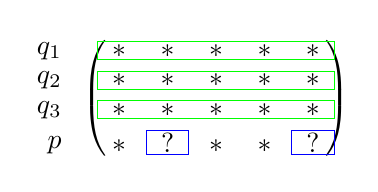
\begin{tikzpicture}[baseline = (M.center),% center with respect to the matrix center
	every left delimiter/.style={xshift=1ex},%tighter delimiter spacing
	every right delimiter/.style={xshift=-1ex}]
	\matrix (M) [matrix of math nodes,
	inner sep=0pt, column sep=0.25em,
	row sep=1pt,
	nodes={inner sep=0.25em,text width=1em,align=center},
	left delimiter=(,right delimiter=),
	]{ 
		* & * & * & * & *  \\
		* & * & * & * & *  \\
		* & * & * & * & *  \\
		* & ? & * & * & ?  \\
	};
	\draw[green!50!green] ([yshift=-1.75pt]M-1-1.north west) rectangle ([yshift=1.75pt]M-1-5.south east);
	\draw[green!50!green] ([yshift=-1.75pt]M-2-1.north west) rectangle ([yshift=1.75pt]M-2-5.south east);
	\draw[green!50!green] ([yshift=-1.75pt]M-3-1.north west) rectangle ([yshift=1.75pt]M-3-5.south east);
	\draw[blue!50!blue] ([yshift=-1.75pt]M-4-2.north west) rectangle ([yshift=1.75pt]M-4-2.south east); 
	\draw[blue!50!blue] ([yshift=-1.75pt]M-4-5.north west) rectangle ([yshift=1.75pt]M-4-5.south east);
	
	\node[anchor=south east, left=6pt] (M-0-0) at (M-1-1.north west) {};
	% iterate over each row and their corresponding labels
	\foreach[count=\i] \v in {\(q_1\),\(q_2\),\(q_3\),\(p\)}{
		% label of this row, based on size of diagonal element
		\node (M-\i-0) at (M-0-0 |- M-\i-\i) {};
		% put the text (specified in the loop) at the label
		\path (M-\i-0.north) -- (M-\i-0.south) node [midway, left] { \v };
	}
	\end{tikzpicture}
\end{document}